\chapter{Introduction and Motivation}

\begin{figure}[h] 
\centering
  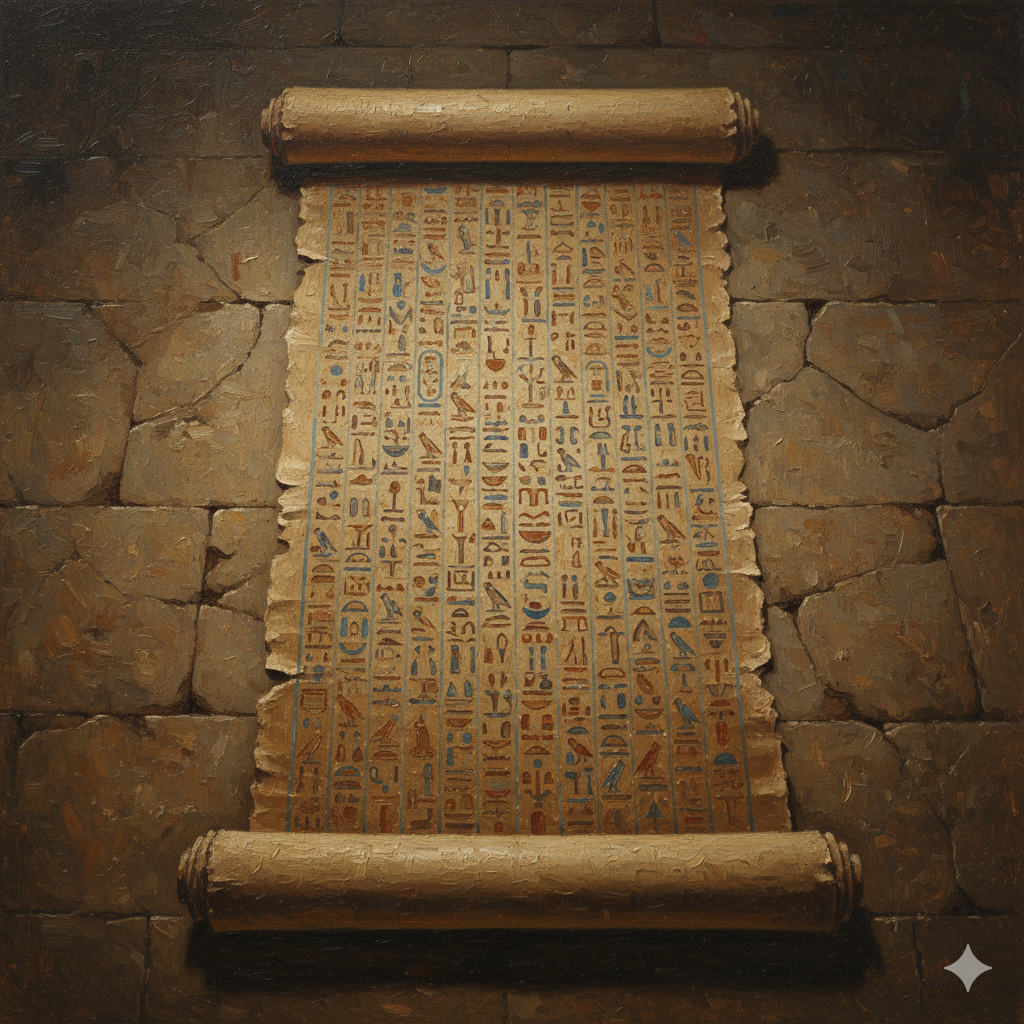
\includegraphics[width=12.5cm]{Abbildungen/hieroglyphs.png}
\caption{An ancient scroll of hieroglyphs.}
\label{fig:hieroglyphs.png}
\end{figure}


This lecture explores the theory of formal languages and delves into various applications, with a focus on the
development of scanners, parsers, interpreters, and compilers. We also introduce a tool designed to aid in the
creation of these components, specifically we will introduce
\href{https://www.dabeaz.com/ply/ply.html}{\texttt{Ply}}, which can be used both as a scanner generator and as
a parser generator. 

\section{Basic Definitions}
The cornerstone of this lecture is the concept of a \href{http://en.wikipedia.org/wiki/Formal_language}{\emph{formal language}}, \index{formal language} essentially defined as a set of strings characterized by precise mathematical criteria. To establish this concept, we first introduce some foundational definitions.

\begin{Definition}[Alphabet]
An \blue{alphabet} \( \Sigma \) \index{alphabet} is a finite, non-empty set of \blue{characters}:
\\[0.2cm]
\hspace*{1.3cm}
\( \Sigma = \{ c_1, \cdots, c_n \} \).
\\[0.2cm]
The term \blue{symbol} \index{symbol} is occasionally used interchangeably with the term \blue{character}.
\eox
\end{Definition}

\examplesEng
\begin{enumerate}[(a)]
\item \( \Sigma = \{ \mathtt{0}, \mathtt{1} \} \) is the alphabet for representing binary numbers.
\item $\Sigma = \{$ ``\texttt{a}'', $\cdots$, ``\texttt{z}'', ``\texttt{A}'', $\cdots$, ``\texttt{Z}'' $\}$ 
      is the standard alphabet for the English language.
\item \( \Sigma_{\textsc{\scriptsize Ascii}} = \{ 0, 1, \cdots, 127 \} \) is known as the
      \href{http://en.wikipedia.org/wiki/ASCII}{\textsc{Ascii}-alphabet}. \index{\textsc{Ascii}-Alphabet} Here,
      numbers correspond to letters, digits, punctuation marks, and control characters. For instance, the set
      of number \( \{ 65, \cdots, 90 \} \) represents the letters \( \{ \texttt{A}, \cdots, \texttt{Z} \} \):
      The number $65$ represents the letter ``\texttt{A}'', the number $66$ represents the letter
      ``\texttt{B}'', and the number $90$ represents the letter ``\texttt{Z}''.
      Table \ref{tab:ascii_table} on the next page shows the complete \textsc{Ascii}-alphabet.  Note that the
      first 32 codes are non-printable control codes, for example the number $10$ encodes a line feed control
      symbol, while the number $13$ encodes a carriage return control symbol.
      
\item \( \Sigma_{\textsc{\scriptsize Unicode}} = \{ 0, 1, \cdots, 159,801 \} \) represents version 17.0 of the
      \href{https://en.wikipedia.org/wiki/Unicode}{\textsc{Unicode}-alphabet}. \index{\textsc{Unicode}-Alphabet}
      This extensive set accommodates a wide array of characters, including various scripts, symbols, and even
      emojis.  Table \ref{tab:chinese_table} shows the Unicode encoding of the 120 most common Chinese characters.
\eox
\end{enumerate}

\begin{table}[!th]
    \centering
    \begin{tabular}{|c|c|c|c|c|c|}
        \hline
        \textbf{Character} & \textbf{Code} & \textbf{Character} & \textbf{Code} & \textbf{Character} & \textbf{Code} \\
        \hline        \hline
                   &    &            &    & \texttt{Space} & 32 \\
        \texttt{!} & 33 & \texttt{"} & 34 & \texttt{\#} & 35 \\
        \texttt{\$} & 36 & \texttt{\%} & 37 & \texttt{\&} & 38 \\
        \texttt{\textquotesingle} & 39 & \texttt{(} & 40 & \texttt{)} & 41 \\
        \texttt{*} & 42 & \texttt{+} & 43 & \texttt{,} & 44 \\
        \texttt{-} & 45 & \texttt{.} & 46 & \texttt{/} & 47 \\
        \texttt{0} & 48 & \texttt{1} & 49 & \texttt{2} & 50 \\
        \texttt{3} & 51 & \texttt{4} & 52 & \texttt{5} & 53 \\
        \texttt{6} & 54 & \texttt{7} & 55 & \texttt{8} & 56 \\
        \texttt{9} & 57 & \texttt{:} & 58 & \texttt{;} & 59 \\
        \texttt{<} & 60 & \texttt{=} & 61 & \texttt{>} & 62 \\
        \texttt{?} & 63 & \texttt{@} & 64 & \texttt{A} & 65 \\
        \texttt{B} & 66 & \texttt{C} & 67 & \texttt{D} & 68 \\
        \texttt{E} & 69 & \texttt{F} & 70 & \texttt{G} & 71 \\
        \texttt{H} & 72 & \texttt{I} & 73 & \texttt{J} & 74 \\
        \texttt{K} & 75 & \texttt{L} & 76 & \texttt{M} & 77 \\
        \texttt{N} & 78 & \texttt{O} & 79 & \texttt{P} & 80 \\
        \texttt{Q} & 81 & \texttt{R} & 82 & \texttt{S} & 83 \\
        \texttt{T} & 84 & \texttt{U} & 85 & \texttt{V} & 86 \\
        \texttt{W} & 87 & \texttt{X} & 88 & \texttt{Y} & 89 \\
        \texttt{Z} & 90 & \texttt{[} & 91 & \texttt{\textbackslash} & 92 \\
        \texttt{]} & 93 & \texttt{\symbol{94}} & 94 & \texttt{\_} & 95 \\
        \texttt{\symbol{96}} & 96 & \texttt{a} & 97 & \texttt{b} & 98 \\
        \texttt{c} & 99 & \texttt{d} & 100 & \texttt{e} & 101 \\
        \texttt{f} & 102 & \texttt{g} & 103 & \texttt{h} & 104 \\
        \texttt{i} & 105 & \texttt{j} & 106 & \texttt{k} & 107 \\
        \texttt{l} & 108 & \texttt{m} & 109 & \texttt{n} & 110 \\
        \texttt{o} & 111 & \texttt{p} & 112 & \texttt{q} & 113 \\
        \texttt{r} & 114 & \texttt{s} & 115 & \texttt{t} & 116 \\
        \texttt{u} & 117 & \texttt{v} & 118 & \texttt{w} & 119 \\
        \texttt{x} & 120 & \texttt{y} & 121 & \texttt{z} & 122 \\
        \texttt{\{} & 123 & \texttt{|} & 124 & \texttt{\}} & 125 \\
        \texttt{\textasciitilde} & 126 & \texttt{DEL} & 127 &  & \\
        \hline
    \end{tabular}
    \caption{\textsc{Ascii} Encoding Table}
    \label{tab:ascii_table}
\end{table}

\begin{CJK}{UTF8}{gbsn} % Start the Chinese environment with simplified Chinese font

\begin{table}[!th]
    \centering
    \begin{tabular}{|c|c|c|c|c|c|c|c|}
    \hline
    \textbf{Glyph} & \textbf{Unicode} & \textbf{Glyph} & \textbf{Unicode} & \textbf{Glyph} & \textbf{Unicode}  & \textbf{Glyph} & \textbf{Unicode} \\
      \hline
    一 & U+4E00 & 二 & U+4E8C & 三 & U+4E09 & 四 & U+56DB \\
    五 & U+4E94 & 六 & U+516D & 七 & U+4E03 & 八 & U+516B \\
    九 & U+4E5D & 十 & U+5341 & 人 & U+4EBA & 大 & U+5927 \\
    天 & U+5929 & 地 & U+5730 & 日 & U+65E5 & 月 & U+6708 \\
    山 & U+5C71 & 水 & U+6C34 & 火 & U+706B & 木 & U+6728 \\
    金 & U+91D1 & 土 & U+571F & 子 & U+5B50 & 女 & U+5973 \\
    中 & U+4E2D & 国 & U+56FD & 王 & U+738B & 民 & U+6C11 \\
    学 & U+5B66 & 文 & U+6587 & 本 & U+672C & 书 & U+4E66 \\
    爱 & U+7231 & 家 & U+5BB6 & 友 & U+53CB & 生 & U+751F \\
    父 & U+7236 & 母 & U+6BCD & 男 & U+7537 & 女 & U+5973 \\
    花 & U+82B1 & 草 & U+8349 & 狗 & U+72D7 & 猫 & U+732B \\
    鸟 & U+9E1F & 鱼 & U+9C7C & 风 & U+98CE & 雨 & U+96E8 \\
    云 & U+4E91 & 雪 & U+96EA & 电 & U+7535 & 光 & U+5149 \\
    车 & U+8F66 & 船 & U+8239 & 米 & U+7C73 & 茶 & U+8336 \\
    饭 & U+996D & 面 & U+9762 & 东 & U+4E1C & 西 & U+897F \\
    南 & U+5357 & 北 & U+5317 & 左 & U+5DE6 & 右 & U+53F3 \\
    高 & U+9AD8 & 矮 & U+77EE & 长 & U+957F & 短 & U+77ED \\
    快 & U+5FEB & 慢 & U+6162 & 早 & U+65E9 & 晚 & U+665A \\
    你 & U+4F60 & 好 & U+597D & 谢 & U+8C22 & 是 & U+662F \\
    不 & U+4E0D & 我 & U+6211 & 他 & U+4ED6 & 她 & U+5979 \\
    它 & U+5B83 & 很 & U+5F88 & 要 & U+8981 & 有 & U+6709 \\
    吃 & U+5403 & 喝 & U+559D & 看 & U+770B & 听 & U+542C \\
    走 & U+8D70 & 跑 & U+8DD1 & 跳 & U+8DF3 & 说 & U+8BF4 \\
    问 & U+95EE & 答 & U+7B54 & 学 & U+5B66 & 校 & U+6821 \\
    老 & U+8001 & 师 & U+5E08 & 生 & U+751F & 书 & U+4E66 \\
    \hline
    \end{tabular}
    \caption{\textsc{Unicode} Encoding of some Chinese Characters}
    \label{tab:chinese_table}
\end{table}
\end{CJK}

\begin{Definition}[Strings]
For a given alphabet \( \Sigma \), a \blue{string} \index{string} is a sequence of characters selected from \( \Sigma \). In formal language theory, these sequences are written without brackets or separating commas. Thus, for \( c_1, \cdots, c_n \in \Sigma \), we write
\\[0.2cm]
\hspace*{1.3cm}
\( w = c_1 \cdots c_n \) \quad instead of \quad \( w = [c_1, \cdots, c_n] \).
\\[0.2cm]
The \blue{empty string}\index{empty string, $\lambda$} is represented by \( \lambda \), \index{\( \lambda \)} so \( \lambda = \texttt{""} \).
The set of all possible strings formed from the alphabet \( \Sigma \) is denoted as \( \Sigma^* \). \index{\( \Sigma^* \)} Strings are often enclosed in quotation marks for emphasis.
\eox
\end{Definition}
\pagebreak

\examplesEng
\begin{enumerate}[(a)]
\item Let \( \Sigma = \{0, 1\} \).  If we define
      \\[0.2cm]
      \hspace*{1.3cm}
      \( w_1 := \mathtt{"01110"} \) and \( w_2 := \mathtt{"11001"} \),
      \\[0.2cm]
      then both \( w_1 \) and \( w_2 \) are strings over \( \Sigma \). Hence, we can state:
      \\[0.2cm]
      \hspace*{1.3cm}
      \( w_1 \in \Sigma^* \) and \( w_2 \in \Sigma^* \).
\item Consider \( \Sigma = \{\mathtt{a}, \cdots, \mathtt{z}\} \). With
      \\[0.2cm]
      \hspace*{1.3cm}
      \( w := \mathtt{"example"} \),
      \\[0.2cm]
      it follows that \( w \in \Sigma^* \). \eox
\end{enumerate}

The \emph{length} of a string \( w \) is denoted by \( |w| \) and represents the number of characters in \( w
\).\index{length of a string}  
We employ \blue{array notation} for character extraction: given a string \( w \) and a natural number
\( i \leq |w| \), \( w[i] \) specifies the \( i \)-th character in \( w \). Character counting starts at 0, adhering to
conventions in modern programming languages like \texttt{C}, \textsl{Java}, and \textsl{Python}. 

Next, we introduce the concept of \blue{concatenation} \index{concatenation} of two strings \( w_1 \) and
\(w_2 \). Concatenation results in a new string \( w \) formed by appending \( w_2 \) to \( w_1 \). It is
represented as \( w_1 \cdot w_2 \).  In most books the concatenation of $w_1$ and $w_2$ is written without the
dot as \( w_1w_2 \). 

\vspace*{0.3cm}

\exampleEng
For \( \Sigma = \{\mathtt{0}, \mathtt{1}\} \) and \( w_1 = \mathtt{"01"} \) and \( w_2 = \mathtt{"10"} \), the concatenated strings are:
\\[0.2cm]
\hspace*{1.3cm}
\( w_1 \cdot w_2 = \mathtt{"0110"} \) and \( w_2 \cdot w_1 = \mathtt{"1001"} \). \eox

\begin{Definition}[Formal Language] \hspace*{\fill} \linebreak
Given an alphabet \( \Sigma \), a subset \( L \subseteq \Sigma^* \) is called a \blue{formal language} if it is
\emph{precisely defined}. \index{formal language} \eox 
\end{Definition}

You may wonder what it means for a subset to be \emph{precisely defined}.  A subset $L$ is precisely defined if
for every $w \in \Sigma^*$ the notion $w \in L$ is unambiguously defined.  For instance, English doesn't
qualify as a formal language because it lacks a precise rule set for valid sentences. 
\vspace*{0.2cm}

The  definition of the concept of a formal language is intentionally broad. As we progress through the lecture,
we will explore specialized 
versions, most notably \href{http://en.wikipedia.org/wiki/Regular_language}{regular languages}
\index{regular language} and \href{http://en.wikipedia.org/wiki/Context-free_language}{context-free
  languages}. \index{context-free language} These are particularly relevant in computer science. 

\examplesEng
\begin{enumerate}
\item Assume that $\Sigma = \{\mathtt{0},\mathtt{1}\}$.  Define
      \\[0.2cm]
      \hspace*{1.3cm}
      $L_\mathbb{N} = \{ \mathtt{1} \cdot w \mid w \in \Sigma^* \} \cup \{ \mathtt{0} \}$
      \\[0.2cm]
      Then $L_\mathbb{N}$ is the language consisting of all strings that can be interpreted as
      natural numbers given in binary notation.  The language contains all strings from $\Sigma^*$  that start with 
      the character \texttt{1} as well as the string \texttt{0}, which only contains the character
      \texttt{0}.  For example, we have
      \\[0.2cm]
      \hspace*{1.3cm}
      $\mathtt{\symbol{34}100\symbol{34}} \in L_\mathbb{N}$, \quad but \quad $\mathtt{\symbol{34}010\symbol{34}} \not\in L_\mathbb{N}$.
      \\[0.2cm]
      Let us define a function 
      \\[0.2cm]
      \hspace*{1.3cm}
      $\textsl{value}: L_\mathbb{N} \rightarrow \mathbb{N}$
      \\[0.2cm]
      on the set $L_\mathbb{N}$.  We define $\textsl{value}(w)$ by induction on the length of $w$.
      We call $\textsl{value}(w)$ the \blue{interpretation} of $w$.  The idea is that
      $\textsl{value}(w)$ computes the number that is represented by the string $w$:
      \begin{enumerate}
      \item $\textsl{value}(\mathtt{0}) = 0$, $\textsl{value}(1) = 1$,
      \item $|w| > 0 \rightarrow \textsl{value}(w\mathtt{0}) = 2 \cdot \textsl{value}(w)   $,
      \item $|w| > 0 \rightarrow \textsl{value}(w\mathtt{1}) = 2 \cdot \textsl{value}(w) + 1$.
      \end{enumerate}
\item Again we have $\Sigma = \{0,1\}$. Define the language $L_\mathbb{P}$
      to be the set of all strings from $L_\mathbb{N}$ that are prime numbers:
      \\[0.2cm]
      \hspace*{1.3cm}
      $L_\mathbb{P} := \{ w \in L_\mathbb{N} \mid \textsl{value}(w) \in \mathbb{P} \}$
      \\[0.2cm]
      Here, $\mathbb{P}$ denotes the set of \blue{prime numbers}, \index{prime number} which is the set of all natural
      numbers $p$ bigger than $1$ that have no divisor other than $1$ or $p$:
      \\[0.2cm]
      \hspace*{1.3cm}
      $\mathbb{P} = \bigl\{ p \in \mathbb{N} \;\big|\; \{ t \in \mathbb{N} \mid \exists k \in
      \mathbb{N} : k \cdot t = p \} = \{1, p\} \bigr\}$.
\item Define $\Sigma_{\textsc{\scriptsize Ascii}} = \{ 0, \cdots, 127\}$.  Furthermore, define $L_C$
      as the set of all strings of the form
      \\[0.2cm]
      \hspace*{1.3cm}
      \texttt{char* $f$(char* $x$) \{ $\cdots$ \}}
      \\[0.2cm]
      that are, furthermore, valid \texttt{C} function definitions.
      Therefore,  $L_C$ contains all those strings that can be interpreted as a \texttt{C} function $f$
      such that $f$ takes a single argument which is a string and returns a value which is also a
      string.
\item Define $\Sigma := \Sigma_{\textsc{\scriptsize Ascii}} \cup \{\dag\}$, where
      $\mathtt{\dag}$ is some new symbol that is different from all symbols in
      $\Sigma_{\textsc{\scriptsize Ascii}}$.
      The \blue{universal language} \index{universal language} $L_u$ is the set of all strings of the form
      \\[0.2cm]
      \hspace*{1.3cm}
      $p$\dag$x$\dag$y$
      \\[0.2cm]
      such that
      \begin{enumerate}
      \item $p \in L_C$,
      \item $x,y \in \Sigma_{\textsc{Ascii}}^*$,
      \item if $f$ is the function that is defined by $p$, then $f(x)$ yields the result $y$.
            \eox
      \end{enumerate}
    \end{enumerate}

The above examples illustrate the expansive scope of what can be considered a formal language. While it's
straightforward to identify strings in \( L_\mathbb{N} \), this becomes substantially more challenging for
languages like \( L_\mathbb{P} \) or \( L_C \). Moreover, since the
\href{https://en.wikipedia.org/wiki/Halting_problem}{halting problem} is undecidable, no algorithm can
definitively determine membership in the universal language \( L_u \). Nevertheless, \( L_u \) is \blue{semi-decidable}: if a string
\( w \) belongs to \( L_u \), we can eventually establish this fact.  

\section{Overview}
The aim of this lecture is to cover a series of interconnected topics.
While this overview will introduce some terms that may not be immediately clear, rest assured that these terms will
be elaborated upon as the lecture progresses.
The lecture is structured into three main parts: 

\begin{enumerate}
\item The first part delves into the theory of \blue{regular languages}.  These are those languages that can be
  described by a \href{https://en.wikipedia.org/wiki/regular_expression}{regular expression}.
  \begin{enumerate}[(a)]
  \item We begin with an exploration of \blue{regular expressions}. After formally defining this term, we will discuss its applications in \textsl{Python}.
  \item We then demonstrate how the \blue{\textsc{Ply}} tool can be utilized to create \blue{scanners}.
  \item Subsequently, we examine the implementation of regular expressions via \blue{finite state machines}.
  \item A discussion on how to verify the \blue{equivalence} of regular expressions follows.
  \item We conclude this section by discussing the limitations of regular languages, focusing particularly on the \blue{Pumping Lemma}.
  \end{enumerate}
  
\item The second part is centered on \blue{context-free languages}, which are instrumental in describing the syntax of programming languages.
  \begin{enumerate}[(a)]
  \item We first introduce \blue{context-free grammars}, which are employed to define context-free languages.
  \item Next, we talk about using \blue{\textsc{Ply}} as a parser generator.
  \item Essential theory for understanding the parser generator \textsc{Ply} is then presented.
  \item Lastly, we discuss the limitations of context-free languages.
  \end{enumerate}

\item The final part of this lecture covers interpreters and compilers.
  \begin{enumerate}[(a)]
  \item We implement an interpreter for a toy language.
  \item Then we discuss how to implement a compiler that translates another toy language into \blue{Java byte code}.
  \end{enumerate}
\end{enumerate}

\section{Literature}
Besides these lecture notes, there are three books I highly recommend:
\begin{enumerate}[(a)]
\item \emph{Introduction to Automata Theory, Languages, and Computation} \cite{hopcroft:06}
      --- Often considered   the definitive text on formal languages, this book encompasses all the theoretical
      concepts discussed in this lecture, although we will only touch on a subset of its content. 
\item \emph{Introduction to the Theory of Computation} \cite{sipser:2012}
      --- This book provides another accessible introduction to formal languages and extends to the theory of
      computability, which is beyond the scope of this lecture. 
\item \emph{Compilers --- Principles, Techniques and Tools} \cite{aho:2006}
      --- A standard reference in compiler theory, this book also covers a substantial portion of formal languages.
\item The large language models \href{https://gemini.google.com/}{Gemini},
      \href{https://grok.com/}{Grok}, \href{https://claude.ai/}{Claude}, \href{https://www.deepseek.com/}{Deepseek},
      and \href{https://chatgpt.com/}{ChatGPT} have reached a level of maturity
      that allows them to serve as a tutor for many concepts discussed in this course.
\end{enumerate}

\section{Check your Understanding}
\begin{enumerate}[(a)]
\item Define the notion of an \blue{alphabet}.
\item Based on a given alphabet, define the concept of a \blue{string}.
\item Explain the concept of a \blue{formal language}.
\end{enumerate}


%%% Local Variables: 
%%% mode: latex
%%% TeX-master: "formal-languages.tex"
%%% End: 
